\documentclass[a4paper, 11pt, hidelinks]{article}
\usepackage[left=2cm, top=3cm, text={17cm, 24cm}]{geometry}
\usepackage[czech]{babel}
\usepackage[utf8]{inputenc}
\usepackage{hyperref}
\usepackage{tabularx}
\usepackage{booktabs}
\usepackage{xcolor}
\usepackage{graphicx}

\bibliographystyle{plain}

\begin{document}

\begin{titlepage}
    \begin{center}
        \Huge \textsc{Vysoké učení technické v~Brně} \\
        \huge \textsc{Fakulta informačních technologií} \\
        \vspace{\stretch{0.382}}
        Síťové aplikace a správa sítí\,--\,monitorování DHCP komunikace\\
        \Huge  Manuál k programu dhcp-stats\\
        \vspace{\stretch{0.618}}
        \Large \today{} \hfill Ondřej Koumar (xkouma02)
    \end{center}
\end{titlepage}

\tableofcontents

\newpage

\section*{Úvod}\label{0_uvod}
\addcontentsline{toc}{section}{Úvod}
Ne vždy má uživatel možnost sledovat statistiku vytížení síťových prefixů.
Některé DHCP servery tuto statistiku poskytují samy, případně se mohou parsovat adresy z jejich logů.
Pokud ale takováto možnost není, nezbývá moc jiných možností, než sledovat DHCP provoz odchytáváním paketů a manuálním parsováním IP adres, které jsou klientským stanicím přidělovány.
To je use-case, pro který byl program \texttt{dhcp-stats} vytvořen.

Program \texttt{dhcp-stats} je schopen monitorovat DHCP provoz na vybraném rozhraní, ať už se jedná o ethernetové či bezdrátové, a generovat statistiku pro uživatelem zadaný síťový prefix.
Samotné monitorování spočívá v odchytávání a filtraci paketů, které na daném rozhraní projdou, a hledání podstatných informací v nich.
V paketu, který je odeslán DHCP serverem, případně klientem, který DHCP službu využívá, jsou umístěny veškeré informace, které jsou potřebné pro generování statistiky pro síťový prefix.

Pokud uživatel nemá potřebu přímo monitorovat DHCP provoz naživo, má možnost využít zpracování \emph{.pcap} nebo \emph{.pcapng} souborů (které si může vygenerovat například pomocí programu Wireshark\footnote{O programu se dozvíte na \href{https://www.wireshark.org/about.html}{https://www.wireshark.org/about.html}.}).
To se hodí například v případě, že má již síť zmonitorovanou a nepotřebuje real-time statistiku.
V tomto případě je ale počítat s tím, že možnosti programu jsou omezené; vypíše se pouze finální podoba sítě, tedy vytížení prefixů v době, kdy skončilo zachytávání paketů.
Je ale možné do programu uměle vložit zpoždění tak, aby šlo vidět zpracování paketů po jednom.
Více o této možnosti v kapitole \ref{3_popis}.

\newpage
\section{Uvedení do problematiky}\label{1_problematika}
DHCP (\emph{Dynamic Host Configuration Protocol}) je popsán v rámci \href{https://datatracker.ietf.org/doc/html/rfc2131}{RFC 2131}. 
DHCP se skládá za dvou částí\,--\,z protokolu zajišťujícího doručování parametrů od serveru ke klientovi a systém alokací IP adres.
Je postaven na modelu klient-server, kde server je zařízení, které poskytuje parametry přes přenosovou část protokolu a klient je zařízení, které o tyto parametry DHCP server žádá.

\subsection{DHCP pakety}\label{1_1_pakety}
Položky DHCP paketu a jejich vysvětlení:
\begin{table}[ht]
  \centering
  \begin{tabularx}{\textwidth}{p{0.1\textwidth}p{0.15\textwidth}p{0.67\textwidth}}
    \toprule
    \textbf{Pole} & \textbf{Velikost (B)} & \textbf{Popis} \\
    \midrule
    \texttt{op} & 1 & Kód operace zprávy. \\
    \texttt{htype} & 1 & Typ hardwarové adresy. \\
    \texttt{hlen} & 1 & Délka hardwarové adresy. \\
    \texttt{hops} & 1 & Počet relay agentů\footnotemark[2], přes které šla DHCP zpráva. \\
    \texttt{xid} & 4 & ID transakce, které používají jak server, tak klient k identifikaci zpráv. \\
    \texttt{secs} & 2 & Počet sekund od začátku transakce (žádost o adresu nebo obnovení \emph{lease time}). \\
    \texttt{flags} & 2 & Příznak broadcastu. \\
    \texttt{ciaddr} & 4 & IP adresa klienta. \\
    \texttt{yiaddr} & 4 & Nová klientova IP adresa (použito při nabízení a potvrzování adres od serveru). \\
    \texttt{siaddr} & 4 & IP adresa serveru, který má klient kontaktovat při další zprávě. \\
    \texttt{giaddr} & 4 & IP adresa relay agenta, přes kterého se posílají DHCP zprávy. \\
    \texttt{chaddr} & 16 & MAC adresa klientovy síťové karty. \\
    \texttt{sname} & 64 & Jméno serveru (volitelné). \\
    \texttt{file} & 128 & Název souboru, který klient použije pro bootstrapping\footnotemark[3]. \\
    \texttt{options} & n & Pole volitelných parametrů.\\
    \bottomrule
  \end{tabularx}
  \label{tab:dhcp-format}
  \caption{Formát zprávy DHCP}
\end{table}

\footnotetext[2]{V kontextu DHCP se jedná o proces získání potřebných informací od DHCP serveru.}
\footnotetext[3]{Relay agenti mají na starost přeposílání paketů mezi klientem a serverem při DHCP komunikaci.}

Poznámky:
\begin{itemize}
    \item \texttt{op} Může nabývat hodnot BOOTREQUEST a BOOTREPLY.
    \item Výčet typů hardwarových adres \href{https://www.iana.org/assignments/arp-parameters/arp-parameters.xhtml#arp-parameters-2}{\textcolor{blue}{zde}}.
    \item \texttt{xid} je náhodné číslo generované klientem, používá se po celou dobu komunikace.
    \item \texttt{flags} je ve formátu: 

        \begin{table}[ht]
            \centering
            \begin{tabular}{|c|c|}
            \hline
            \textbf{Bits} & \textbf{Value} \\
            \hline
            0             & B \\
            1-15          & MBZ \\
            \hline
            \end{tabular}
            \caption{\texttt{flags} pole}
            \label{tab:dhcp_flags}
        \end{table}
        
        kde \emph{B} je příznak, že zpráva byla poslána na broadcastovou adresu sítě, \emph{MBZ} je 15 bitů, které jsou vždy nastaveny na 0.
    \item \texttt{options} je proměnné velikosti, klient ale musí být připraven přijmout DHCP zprávu, která má velikost \texttt{options} alespoň 312\,B.
    Ne všechny parametry se do pole \texttt{options} musí vlézt; pokud je třeba, DHCP server může využít pole \texttt{sname} případně pole \texttt{file} pro uložení zbývajících parametrů.
    Pro výčet parametrů, které se v tomto poli mohou vyskytnout, vizte \href{https://www.iana.org/assignments/bootp-dhcp-parameters/bootp-dhcp-parameters.xhtml#options}{\textcolor{blue}{zde}}.
\end{itemize}

\subsection{DHCP komunikace}\label{1_2_komunikace}

\subsubsection{DHCP zprávy}\label{1_2_1_zpravy}

Před vysvětlením samotné komunikace je potřeba základní výčet zpráv, které si klient a server v rámci DHCP posílají.

\begin{table}[h]
    \centering
    \begin{tabularx}{\textwidth}{lX}
        \toprule
        \textbf{Zpráva} & \textbf{Využití} \\
        \midrule
        DHCPDISCOVER & Klientovo vysílání pro nalezení dostupných serverů. \\
        DHCPOFFER & Odpověď serveru na DHCPDISCOVER s nabídkou konfiguračních parametrů. \\
        DHCPREQUEST & Může mít několik různých významů:
        \begin{itemize}
            \item Klient nemá problém s nabídnutými parametry v DHCPOFFER, zažádá o ně tedy v rámci této zprávy.
            \item Klient se ptá na správnost dříve přidělené adresy po např. restartu systému.
            \item Klient chce prodloužit pronájem (\emph{lease time}) již používané síťové adresy.
        \end{itemize}
        Kompletní přehled a více informací \href{https://www.freesoft.org/CIE/RFC/2131/24.html}{\textcolor{blue}{zde}}. \\
        DHCPACK & Posílá server, obsahuje konfigurační parametry (\ref{tab:dhcp-format}) pro klienta do sítě. \\
        DHCPNAK & Posílá server, oznamuje, že server nesouhlasí s parametry, o které si klient zažádal v DHCPREQUEST. \\
        DHCPDECLINE & Posílá klient a oznamuje, že IP adresa je již používána. \\
        DHCPRELEASE & Posílá klient, ruší pronájem IP adresy (z různých důvodů). \\
        DHCPINFORM & Posílá klient a ptá se, jaké má lokální konfigurační parametry, přičemž adresa mu již byla přidělena externě. \\
        \bottomrule
    \end{tabularx}
    \caption{Typy DHCP zpráv a jejich využití}
    \label{tab:dhcp_messages}
\end{table}

\subsubsection{Posloupnost zpráv}\label{1_2_2_posloupnost}

Komunikaci začíná klient tím, že na obecný broadcast\footnote[4]{Protože klient nezná prefix lokální sítě, je zvolena adresa, které rozumí všechna zařízení, a to 255.255.255.255.} vyšle DHCPDISCOVER zprávu.
DHCP server tuto zprávu přečte, podívá se na adresy, co má k dispozici a zprávou DHCPOFFER nabídne novému klientovi síťovou konfiguraci.
Také do této zprávy na políčko \texttt{siaddr} vloží svoji IP adresu, aby mohl být server identifikován po zaslání DHCPREQUEST na broadcast.

Klient se na konfiguraci podívá a pokud mu vyhovuje, oficiálně o tuto konfiguraci zažádá zprávou DHCPREQUEST.
Server může přijmout žádost, a tedy poslat potvrzovací DHCPACK zprávu, nebo odmítnout a poslat DHCPNAK zprávu.

V prvním případě má klient ještě možnost odmítnout zprávou DHCPDECLINE, pokud adresu již některé zařízení v síti používá.
V tomto případě se klient vrací do stavu, kdy komunikace se serverem probíhá od začátku zprávou DHCPDISCOVER.
Pokud ne, adresu přijme a může ji používat v lokální síti.
Další komunikace proběhne až klient bude rušit pronájem adresy (případně při zprávě DHCPINFORM).

V druhém případě se klient vrací do fáze, kdy znovu vysílá DHCPDISCOVER zprávu a komunikace se serverem probíhá od začátku.

\begin{figure}[h]
    \centering
    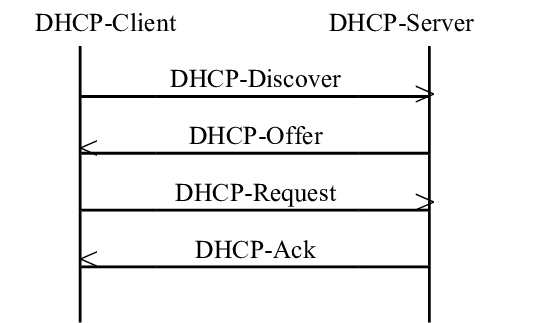
\includegraphics[width=0.6\textwidth]{img/Typical-DHCP-sequence.png}
    \caption{Typická posloupnost DHCP zpráv s jedním serverem.\cite{dhcp-message-sequence}}
    \label{pic:dhcp_sequence}
\end{figure}

Nezapomeňme, že v dosahu se DHCP serverů může vyskytovat více; klient si v tom případě zvolí jeden z nich a jeho adresu vloží do pole \texttt{siaddr}, aby se server mohl identifikovat.
DHCPREQUEST je také posílán na obecný broadcast a servery musí vědět, komu zpráva patří.
Pokud DHCPREQUEST není určen serveru, pak jeho komunikace v tomto bodě končí.

Po vypršení \emph{lease time}, jenž je v DHCP packetu v poli \texttt{options} s číslem 51, případně pokud se klient sám rozhodne z jiných důvodů zrušit pronájem IP adresy, klient posílá zprávu DHCPRELEASE.
Typicky klient kontaktuje stejný server\footnote[5]{Opět na broadcast, tentokrát ale lokální sítě.} zprávou DHCPREQUEST se stejnou adresou, jako používal do této chvíle.
Server může přijmout, a tedy zaslat DHCPACK, případně odmítnout a klient započíná proces získávání IP adresy od začátku zprávou DHCPDISCOVER.
\section{Návrh aplikace}\label{2_navrh}
Aplikace je objektově orientovaná, a proto je implementována v C++.
V aplikaci jsou 4 třídy:
\begin{itemize}
    \item \textbf{ArgumentProcessor} má za úkol zpracovávat argumenty příkazové řádky, které byly programu předány. Kontroluje pouze správnost přepínačů a návratovou hodnotu od IpAddressParseru.
    \item \textbf{IpAddressParser} je pomocníkem ArgumentProcessoru. Z Argumentů příkazové řádky kontroluje správnost IP adres, které byly programu předány. 
    \item \textbf{PacketSniffer} uchovává informace o použitém rozhraní, případně souboru, ze kterého se načítá, dále data a hlavičky paketů a další pomocné struktury potřebné pro čtení paketů.
    Extrahuje IP adresy z paketu a předává je IpAddressManageru.
    \item \textbf{IpAddressManager} je hlavní datovou strukturou programu.
    Uchovává si informace o každé síti, která byla předána jako argument příkazové řádky. 
    Podporuje přidávání i odebírání adres ze sítí.
\end{itemize}\newpage
Dále se v aplikaci nachází datová struktura \textbf{NetworkData}. 
V této struktuře jsou uchovávány veškeré parametry sítě, například:
\begin{itemize}
    \item adresa,
    \item maska,
    \item broadcastová adresa,
    \item počet obsazených adres,
    \item obsazené adresy,
    \item obsazenost v \% a další.
\end{itemize}
S vektorem těchto datových struktur pracuje IpAddressManager.

Program je uzpůsoben tomu, aby při přijmutí signálů \emph{SIGINT} a \emph{SIGTERM} byl bezpečně ukončen. 
Vypisování informací o sítích je řešeno knihovnou ncurses. 
Při překročení 50\,\% vytížení prefixu se standardní logovací rutinou \texttt{syslog} zaloguje tato informace do systémového logu.
Detailnější popis v sekci \ref{3_popis}.

\section{Popis implementace}\label{3_popis}
Program je spuštěn funkcí \texttt{main}, která se nachází v souboru \emph{dhcp-stats.cpp}. 
Volá ArgumentProcessor pro zpracování argumentů, poté PacketSniffer, aby začal zpracovávat pakety na rozhraní, případně v souboru.

\subsection{ArgumentProcessor}\label{3_1_ap}

\subsection{IpAddressParser}\label{3_2_ipap}

\subsection{PacketSniffer}\label{3_3_ps}

\subsection{IpAddressManager}\label{3_4_ipam}

\section{Základní informace o programu}\label{4_zakladni_info}

\section{Návod na použití}\label{5_navod}

\newpage

\bibliography{references}

\end{document}
